\documentclass[11pt,letterpaper,fleqn]{article}
% Inclusion de los paquetes necesarios

\usepackage[latin1]{inputenc}  % Para los caracteres tildados
%\usepackage[utf8]{inputenc}   % Para los caracteres tildados
%If your LaTeX compiler complains about utf8, try utf8x instead.
\usepackage[spanish]{babel}

\usepackage{amsmath,amsfonts}  % Fonts y macros de la American Math Society
\usepackage{amssymb, amsfonts, latexsym, cancel}
\usepackage{geometry}          % margenes de la manera facil
\usepackage{setspace}
\usepackage{hhline}
\usepackage{times}
\usepackage{color}
%\usepackage[sc]{mathpazo}
\usepackage{url}
\usepackage{fancyhdr}          % Fancy Header and Footer
\usepackage[ruled]{algorithm}       
\usepackage{algorithmic}
\usepackage{supertabular}
\usepackage{array}
\usepackage{abstract}
\usepackage{multicol}
\usepackage{titling}
\usepackage{titlesec}
\parindent=0pt

%\usepackage{setspace}          %para manejar single & double space
\usepackage{subfigure}

%~~~~~~~~~~~~~~~~~~~~~~~~~~~~~~~~~~~~~~~~~~~~~~~~~~~~~~~~~~~~~~~~~~~~~~~~~~~~  
%      PLEASE DO NOT MODIFY
%      POR FAVOR NO CAMBIAR

%~~~~~~~~~~~~~~~~~~~~~~~~~~~~~~~~~~~~~~~~~~~~~~~~~~~~~~~~~~~~~~~~~~~~~~~~~~~  
% Define the margins

\geometry{verbose, top=1.78cm,bottom=1.78cm, left=2cm, right=1.65cm}
\headheight=.76cm
\headsep=0pt

%~~~~~~~~~~~~~~~~~~~~~~~~~~~~~~~~~~~~~~~~~~~~~~~~~~~~~~~~~~~~~~~~~~~~~~~~~~~ % For use with PDFLaTeX
  \usepackage[pdftex]{graphicx} 
  \pdfcompresslevel=9 
  \usepackage[pdftex,bookmarksopen,colorlinks,linkcolor=blue,%
              citecolor=blue, urlcolor=blue]{hyperref} 

%~~~~~~~~~~~~~~~~~~~~~~~~~~~~~~~~~~~~~~~~~~~~~~~~~~~~~~~~~~~~~~~~~~~~~~~~~~
%   DEFINITIONS



\newcommand{\bx}{\mathbf{x}}
\newcommand{\bu}{\mathbf{u}}
\newcommand{\bd}{\mathbf{d}}
\newcommand{\by}{\mathbf{y}}
\newcommand{\bv}{\mathbf{v}}
\newcommand{\bbf}{\mathbf{f}}

\AtBeginDocument{\renewcommand{\abstractname}{}}

\def\Real{\mathbb{R}}%
\DeclareMathOperator{\volume}{volume}

%~~~~~~~~~~~~~~~~~~~~~~~~~~~~~~~~~~~~~~~~~~~~~~~~~~~~~~~~~~~~~~~~~~~~~~~~~~
%     SECTION FORMAT
\mathindent=10pt
\makeatletter
\abovecaptionskip=4pt
\renewcommand{\section}{\@startsection%
   {section}%
   {1}%
   {\z@}%
   {-\baselineskip}%
   {0.2\baselineskip}%
   {\bfseries\boldmath\MakeUppercase}}
\def\subsection{\@startsection%
   {subsection}%
   {2}%
   {\z@}%
   {-\baselineskip}%
   {0.2\baselineskip}%
   {\noindent\normalsize\boldmath\emph}}
\def\subsubsection{\@startsection{subsubsection}
   {3}
   {\z@}%
   {-13dd plus-4pt minus-4pt}
   {-5.5pt}
   {\normalsize\emph}}

\renewcommand\paragraph{\@startsection{paragraph}{3}{\z@}%
            {-2.5ex\@plus -1ex \@minus -.25ex}%
            {1.25ex \@plus .25ex}%
            {\normalfont\normalsize\bfseries}}

\makeatother
\setcounter{secnumdepth}{3} % how many sectioning levels to assign numbers to
\setcounter{tocdepth}{3}    % how many sectioning levels to show in ToC

%~~~~~~~~~~~~~~~~~~~~~~~~~~~~~~~~~~~~~~~~~~~~~~~~~~~~~~~~~~~~~~~~~~~~~~~~~~~~~~
\begin{document}

\noindent\rule{18cm}{0.4pt}

\noindent
{\LARGE {\textbf{An automation approach of the mechanical design and manufacturing of ball mills}}}
\vspace{.5em}

\noindent 
\large{\textbf{{Juan D. Arguello$^{a*}$, Omar A. G\'elvez$^b$, Jairo R. Mart\'inez$^c$, Diego C. Dur\'an$^c$, Elena E. Stashenko$^c$}}}
\vspace{.3em}

\noindent	
{\small {\emph{$^a$Universidad Industrial de Santander, Escuela de Ingenier�a Mec�nica, Centro Nacional de Investigaciones para la Agroindustrializaci�n de Especies Vegetales Arom�ticas y Medicinales Tropicales - CENIVAM. Bucaramanga, Colombia.}}}

\noindent	
{\small {\emph{$^b$Universidad Industrial de Santander, Escuela de Ingenier�a Mec�nica, Grupo de Investigaci�n en Energ�a y Medio Ambiente - GIEMA. Bucaramanga, Colombia.}}}

\noindent	
{\small {\emph{$^c$Universidad Industrial de Santander, Escuela de Qu�mica, Centro de Investigaci�n en Biomol�culas - CIBIMOL y Centro Nacional de Investigaciones para la Agroindustrializaci�n de Especies Vegetales Arom�ticas y Medicinales Tropicales - CENIVAM. Bucaramanga, Colombia.}}}

%~~~~~~~~~~~~~~~~~~~~~~~~~~~~~~~~~~~~~~~~~~~~~~~~~~~~~~~~~~~~~~~~~~~~~~~~~~~~~~
% The Title -- Titulo     
%  START HERE
%  COMIENCE ACA
%~~~~~~~~~~~~~~~~~~~~~~~~~~~~~~~~~~~~~~~~~~~~~~~~~~~~~~~~~~~~~~~~~~~~~~~~~~~~~~

%~~~~~~~~~~~~~~~~~~~~~~~~~~~~~~~~~~~~~~~~~~~~~~~~~~~~~~~~~~~~~~~~~~~~~~~~~~~~~~
% The Abstract  --  Resumen
%~~~~~~~~~~~~~~~~~~~~~~~~~~~~~~~~~~~~~~~~~~~~~~~~~~~~~~~~~~~~~~~~~~~~~~~~~~~~~~

\noindent\rule{18cm}{0.4pt}

\vspace*{-3.15 em}

\begin{abstract}

\begin{abstractname}

\centering

\large{\textbf{Abstract}}

\end{abstractname}

\vspace{1 em}


   {\small{%
  
Engineering design is taking a new step forward with technological advances. \textit{Open source} tools, such as Python, make it possible to develop calculation and validation algorithms to automate design procedures. Ball mills stands out as a solution for crushing processes, specially in the civil industry, which its design procedure requires the study of the cynematic of the balls and the dynamical interaction between them and the mill. Numerical simulations are usually used as a validation tool, but also as an optimization one. For this particular case, there were used two numerical methods: the \textit{Discrete Element Method} (DEM), used to validate the cynematic theoretical study, optimize it and to predict the impact distribution energy over the mill; and the \textit{Finite Element Method} (FEM), which was used to predict, and guarantee, an adecuate structural behaviour of the mill. The present work also create automatic engineering reports (both in TeX and PDF formats), CAD drawings of the designed ball mill (dxf format) and an automatic quantification of the required materials for manufacturing. All of the above can be summarized in three principal stages, or chapters: the first one is related to the theoretical study, the second one to the numerical simulations and the last one to the obtained results.
   }} 
   
   \vspace{.5 em}

\textit{Keywords:}  {\small{ball mill, automation, mechanical design, FEM, DEM, FEniCS, Python.
}}


\end{abstract}

\vspace{-1em}

\noindent\rule{18cm}{0.4pt}

%~~~~~~~~~~~~~~~~~~~~~~~~~~~~~~~~~~~~~~~~~~~~~~~~~~~~~~~~~~~~~~~~~~~~~~~~~~~~~~
\renewcommand{\arraystretch}{1.3}

\begin{multicols}{2}

\section{Introduction} 

\subsection{Background and Motivation}

In recent years, there have been reported several studies where automation has been used in engineering design. For the production of nuclear energy, it can be found different studies, such as: the design of reactor cores$^{[1]}$, from where Hyun Kim \textit{et al} uses an artificial neural network to provide, and evaluate, new types of geometries; Nomen \textit{et al} developed a numerical methodology to create the design of IFMIF LIPAc beam dump shielding$^{[2]}$, which provides an acelerator-based, D-Li neutron source to produce energy of high intensity by radiation; Kim J. \textit{et al} created an autonomous operation system$^{[3]}$ with artificial intelligence which perform the control functions needed for the emergency operation of a nuclear power plant.


    In civil engineering, there is a specialized journal known as "Automation in Construction", which has published different studies related to automatic structural and seismic designs. In mechanical design, it can be found articles related with automation in different industries, like automotive, fluid transport and robotics, to name a few. For example: Ouyang T. \textit{et al} developed a dynamic modelling of a clutch actuator for heavy duty transmission$^{[4]}$ adopting an artificial bee colony (ABC) algorithm to optimize structural parameters; X. Telleria \textit{et al} presented a methodology to automate the design, and numerical validation, of valves$^{[5]}$; M. Honarpardaz \textit{et al} introduced the Generic Automated Finger Design$^{[6, 7]}$ (GAFD) method for design automation of customized fingers of industrial grippers for robots. 

   Most of these works are intended to study a particular stage of the design, either modelling, numerical method or simulation. The motivation of doing this work was to propose a design methodology, which groups all of this efforts, focusing in the required information for the manufacturing of the mill.
   
\subsection{Future Updates}

Things can always be done better or differently. The main idea of this work was to prove a design methodology, but the possibility to do things "simpler" from the user perspective is still there. To achieve this, an artificial intelligence algorithm must be implemented. 

    Another future update should let advanced users to implement experimental grinding equations to predict time consuming.

\section{Theoretical study}

The goal of this section is to find:

\begin{itemize}
	\item Power.
	\item Diameter of the mill.
	\item Length of the mill.
	\item Rotational speed.
	\item Number of balls.
\end{itemize}

\subsection{Requirements and Specifications}

The \textit{default} requirements data can be appreciated in Table \ref{req}.

\begin{table}[H]
\centering
\begin{tabular}{cc}
\hline
\textbf{Requirements} & \textbf{Value} \\ \hline \hline
Capacity of the mill $[kg/batch]$ & 200 \\ 
Input particle size $\left[\mu m \right]$ & 850 \\
Target particle size $\left[\mu m \right]$ & 250 \\ \hline
\end{tabular}
\caption{\textit{Default} requirements data.}
\label{req}
\end{table}

The \textit{default} specifications data is shown on Table \ref{spec}.

\begin{table}[H]
\centering
\begin{tabular}{cc}
\hline
\textbf{Specifications} & \textbf{Value} \\ \hline \hline
Length - diameter relation & 1.5 - 3 \\ 
Density of balls $\left[kg / m^3 \right]$ & 2700 \\
Density of grinding material $\left[kg / m^3 \right]$ & 2520 \\ 
Occupied volume by the material $[\%]$ & 40 - 60 \\
Occupied volume by the balls $[\%]$ & 10 - 30 \\
Rotational speed criteria $[\%]$ & 80 \\
Safety factor & 2 - 4 \\ \hline
\end{tabular}
\caption{\textit{Default} specifications data.}
\label{spec}
\end{table}

\subsection{Mill volume $\rightarrow$ Diameter and Length}

The mill volume, shown on Figure \ref{volume}, is directly proportional to the sum of the volumes occupied by the grinding material and the balls. It is indirectly proportional to the volume ratio of \textit{all} of the material.

\begin{figure}[H]
\centering
\includegraphics[width=0.5\textwidth]{Images/Preprocesamiento/volumen.PNG}
\caption{Relation between mass and volume.}
\label{volume}
\end{figure}

\begin{equation}
V = \frac{V_{Gm} + V_{Tb}}{P}
\label{VT}
\end{equation}

From Equation \ref{VT}, $V$ is the volume of the mill, $V_{Gm}$ is the volume occupied by the grinding material, $V_{Tb}$ correspond to the total volume occupied by the balls and $P$ is the percentage of the mill volume occupied by the load.

\vspace{.5em}

Replacing the data shown on Tables \ref{req} and \ref{spec} on the Equation \ref{VT}, the \textbf{total volume} of the mill is $416.67 [L]$.

\vspace{.5em}

The volume occupied by the grinding material $V_{Gm}$ and by \textit{all} of the balls $V_{Tb}$ can be appreciated on Table \ref{volumes}.

\begin{table}[H]
\centering
\begin{tabular}{cc}
\hline
\textbf{Type} & \textbf{Value $[L]$} \\ \hline \hline
$V_{Gm}$ & 166.67 \\
$V_{Tb}$ & 41.67 \\
$V_{T}$ & 416.67 \\ \hline
\end{tabular}
\caption{Volume distribution.}
\label{volumes}
\end{table}

Knowing the volume of the mill, the length and diameter can be calculated as follows:
\begin{equation}
V = \frac{\pi}{4} D^2 L
\label{volCil}
\end{equation}

According to Equation \ref{volCil}, the diameter $D$ has a value of $0.71 [m]$ and the length of the mill $L$ is $1.06[m]$.

\subsection{Rotational speed of the mill}

The analysis to define the optimum rotational speed is based on the principle that the minimum rotational speed should made the balls adhered to the surface of the mill.

\begin{figure}[H]
\centering
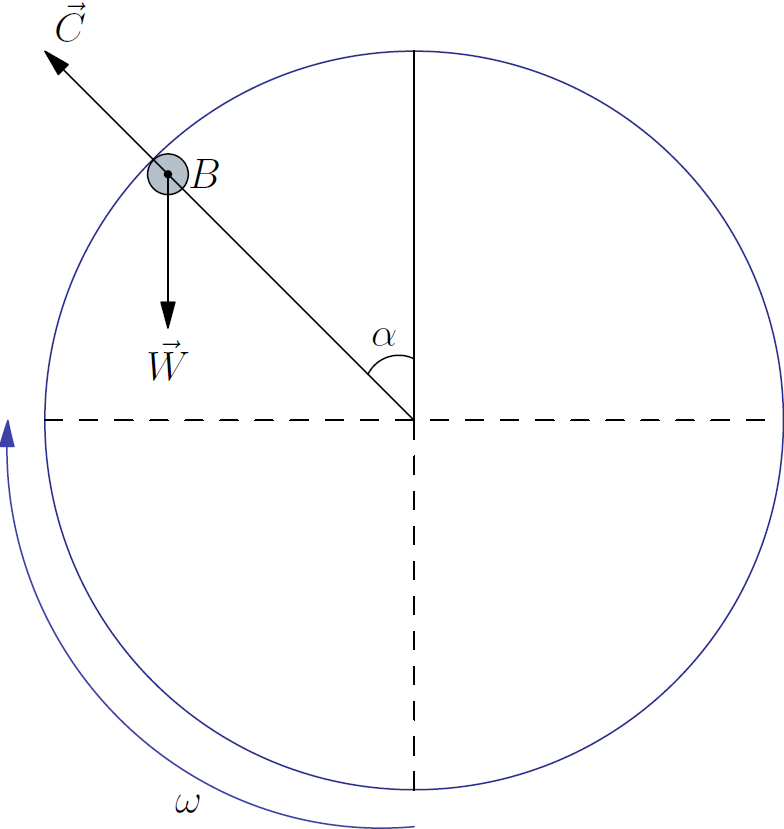
\includegraphics[width=0.5\textwidth]{Images/Preprocesamiento/DBola.PNG}
\caption{Dynamic of a ball.}
\label{DBall}
\end{figure}

Sum of forces in the radial direction gives:

\begin{equation}
\begin{array}{c}
        \sum F_r = 0 = C - W cos \, \alpha \\
        \rightarrow \boxed{C = W cos \, \alpha}
        \label{Fr}
\end{array}
\end{equation}

The dynamic of the ball is defined by:

\begin{equation}
        \vec{C} = m \vec{a_p} 
        \label{dinB}
\end{equation}

Where: $m$ is the mass of the ball and $\vec{a_p}$ is the acceleration vector. The absolute acceleration is equivalent to the sum of three accelerations: rotational acceleration, relative acceleration and the Coriolis acceleration.

\begin{equation}
        \vec{a_p} = \dot{\vec{\omega}} \times \vec{r} + \vec{\omega} \times \left(\vec{\omega} \times \vec{r} \right) + 2 \vec{\omega} \times \left(\dot{\vec{r}} \right) _{rot} + \left(\ddot{\vec{r}} \right) _{f}
        \label{apG}
\end{equation}

The rotational speed of the mill is constant, which implies that the acceleration of the particle behaves as shown on Equation \ref{ap}.

\begin{equation}
        \vec{a_p} = \vec{\omega} \times \left(\vec{\omega} \times \vec{r} \right)
        \tag{6}
        \label{ap}
\end{equation}

Relating Equations \ref{Fr}, \ref{dinB} and \ref{ap}:

\begin{equation}
\begin{array}{c}
        C = W cos \, \alpha = m \left(\omega ^2 r \right) = \left(\frac{W}{g} \right) \left[ \left(\frac{V}{r} \right) ^2 r \right]  \rightarrow \\
        W cos \, \alpha = \frac{W \left(2\pi r N(\alpha) \right)^2}{rg} \rightarrow \boxed{N(\alpha) = \sqrt{\frac{g cos \, \alpha}{4 \pi ^2 r}}}
        \tag{7}
        \label{Nalpha}
\end{array}
\end{equation}

Comparing Equation \ref{Nalpha} with Figure 2, it can be seen that the maximum value of the velocity that the mill should rotate is reached when $\alpha = 0$.

\begin{equation}
        N_{max} = \sqrt{\frac{g}{4 \pi ^2 r}}
        \tag{8}
        \label{N}
\end{equation}

Replacing data shown on Tables \ref{req} and \ref{spec} on Equation \ref{N}, the critical rotational speed $N_{max}$ is of $0.838[rev/s] \rightarrow 50.298[rpm]$. So, the rotational speed $N$ of the mill is $40.24[rpm]$.

\subsection{Number of balls}

The user can specify the diameter of the balls, and how many types there shloud be. The number of balls is calculated by the Equation \ref{Nb}. It has, by default, two types of balls: $2 [cm]$ and $4 [cm]$.

\begin{equation}
        N_b = \frac{V_{Tb}/2}{\frac{4}{3}\pi \left(\frac{D_b}{2} \right) ^2}
        \tag{9}
        \label{Nb}
\end{equation}

Replacing the corresponding data on Equation \ref{Nb}, the number of balls per diameter is:

\begin{itemize}
	\item $2.0[cm] \rightarrow 49$
	\item $4.0[cm] \rightarrow 12$
\end{itemize}

\end{multicols}

\end{document}